\PassOptionsToPackage{table,dvipsnames}{xcolor}
\documentclass[Warsaw]{beamer}

\mode<presentation>
{
	%define logos
	\pgfdeclareimage[width=56.34pt,height=12pt,interpolate=true]{pwrlogo}{pwrlogo}
	\pgfdeclareimage[height=46.48pt,interpolate=true]{pwrlogoduze}{pwrlogoduze}
%	\pgfdeclareimage[width=32pt,height=46.48pt,interpolate=true]{gfxtop}{top}
	%define pwr colors
	\definecolor{pwrdark}{RGB}{156,48,28}
	\definecolor{pwrlight}{RGB}{242,198,140}
	\definecolor{pwrtextonlight}{RGB}{138,47,29}
	\definecolor{niebieski}{RGB}{0,0,254}
	\definecolor{zloty}{RGB}{168,153,110}

	\definecolor{ntnublue}{RGB}{156,48,28}
	%define theme
  \usetheme{boxes}
  \useoutertheme[footline=institutetitle]{miniframes}  
  \useinnertheme[shadow]{rounded}
  \setbeamercovered{transparent}
  %hide navigation symbols
  \setbeamertemplate{navigation symbols}{}	
  %change colors
  \usecolortheme[named=pwrdark]{structure}
  \setbeamercolor{separation line}{bg=pwrdark}
  \setbeamercolor*{titlelike}{parent=palette primary}  
	\setbeamercolor*{palette primary}{use=structure,fg=white,bg=structure.fg}  
  
	%set block colors
\setbeamercolor{block title}{fg=white,bg=ntnublue}
\setbeamercolor{block title alerted}{use=alerted text,fg=white,bg=alerted text.fg!75!black}
\setbeamercolor{block title example}{use=example text,fg=white,bg=zloty}

\setbeamercolor{block body}{parent=normal text,use=block title,bg=block title.bg!15!bg}
\setbeamercolor{block body alerted}{parent=normal text,use=block title alerted,bg=block title alerted.bg!15!bg}
\setbeamercolor{block body example}{parent=normal text,use=block title example,bg=block title example.bg!15!bg}
	
	%define headline with pwr logo
	\defbeamertemplate*{headline}{infolines theme modified by boban}
	{
  \leavevmode%  
  \hbox{%
  \begin{beamercolorbox}[wd=.1\paperwidth,ht=5.25ex,dp=1ex,left]{section in head/foot}%
    \usebeamerfont{section in head/foot}\hspace*{2ex} \pgfuseimage{pwrlogo} \hspace*{2ex}
  \end{beamercolorbox}%
  \begin{beamercolorbox}[wd=.4\paperwidth,ht=2.25ex,dp=1ex,right]{section in head/foot}%
    \usebeamerfont{section in head/foot}\insertsectionhead
  \end{beamercolorbox}%
  \ifx\insertsubsection\empty
     % it is empty
  \else
    \hspace*{2ex}>>
  \fi
  \begin{beamercolorbox}[wd=.4\paperwidth,ht=2.25ex,dp=1ex,left]{subsection in head/foot}%
    \usebeamerfont{subsection in head/foot}\hspace*{2ex}\insertsubsectionhead
  \end{beamercolorbox}}%
  \vskip0pt%
	  \vskip0pt%
	  \begin{beamercolorbox}[colsep=0.5pt]{lower separation line foot}
	  \end{beamercolorbox}
	}

	%define frametitle
	\setbeamercolor{frametitle}{bg=pwrlight}
	\setbeamercolor{frametitle}{fg=pwrdark}
	\setbeamertemplate{frametitle}
	{\vskip-3pt
	  \leavevmode
	  %\hbox{%
	  \begin{beamercolorbox}[wd=\paperwidth,ht=2.4ex,dp=1ex]{frametitle}%
	    \raggedright\hspace*{2em}\textbf\insertframetitle
	  \end{beamercolorbox}%
	 % }%
	  \vskip-11pt%
	  \begin{beamercolorbox}[wd=\paperwidth,colsep=0.5pt]{lower separation line foot}
	  \end{beamercolorbox}%
	  \vskip0pt
	}

	%define footer with page numebers
	\setbeamercolor{foot}{bg=pwrlight}
	\defbeamertemplate*{footline}{infolines theme modified by boban}
	{
	  \leavevmode%
	  \begin{beamercolorbox}[colsep=0.5pt]{upper separation line foot}
	  \end{beamercolorbox}
	  \hbox{%
	  \begin{beamercolorbox}[wd=.33333\paperwidth,ht=2.25ex,dp=1ex,left]{author in head/foot}%
	    \usebeamerfont{author in head/foot}\insertshortauthor~~\insertshortinstitute
	  \end{beamercolorbox}%
	  \begin{beamercolorbox}[wd=.333333\paperwidth,ht=2.25ex,dp=1ex,center]{title in head/foot}%
	    \usebeamerfont{date in head/foot}\insertshortdate{} 
	  \end{beamercolorbox}%
	  \begin{beamercolorbox}[wd=.33333\paperwidth,ht=2.25ex,dp=1ex,right]{date in head/foot}%
	    \hspace*{2em}
	    \insertframenumber{} / \inserttotalframenumber\hspace*{2ex} 
	  \end{beamercolorbox}}%
	  \vskip0pt%
	  \begin{beamercolorbox}[colsep=0.5pt]{lower separation line foot}
	  \end{beamercolorbox}
	}
	
}

\titlegraphic{\pgfuseimage{pwrlogoduze}}


%\usepackage{color}
\usepackage[table,dvipsnames]{xcolor}
%\usepackage{booktabs}
\usepackage[polish]{babel}
%\usepackage{polski}
\usepackage[utf8]{inputenc}
\usepackage[T1]{fontenc}
\usepackage{amsmath}
\usepackage{graphics}
\usepackage{multicol}
%\usepackage{graphicx}
\usepackage{fancyvrb}
\usepackage{listings}
\usepackage{fancyvrb}
\usepackage{parcolumns}
\usepackage{fixltx2e}
\usepackage{multirow}
\usepackage{multicol}
\usepackage{tikz}
\usepackage{tkz-kiviat} 
\usepackage{pmboxdraw}
\usepackage{sectsty}
\usetikzlibrary{arrows}

\newcommand{\todo}[1]{{\color{purple}\textbf{Note: }{#1}}}

\lstset{literate={ą}{{\k{a}}}1 {ć}{{\'c}}1 {ł}{{\l{}}}1 {ń}{{\'n}}1 {ę}{{\k{e}}}1 {ś}{{\'s}}1 {ż}{{\.z}}1 {ó}{{\'o}}1 {ź}{{\'z}}1 {Ą}{{\k{A}}}1 {Ć}{{\'C}}1 {Ł}{{\L{}}}1 {Ń}{{\'N}}1 {Ę}{{\k{E}}}1 {Ś}{{\'S}}1 {Ż}{{\.Z}}1 {Ó}{{\'O}}1 {Ź}{{\'Z}}1 }

\lstdefinelanguage{wccl}
{morekeywords={apply,match,optional,actions,oneof,seq,option,cond},
  sensitive=false,
  keywordstyle=\color[rgb]{0,0,1},
  commentstyle=\color[rgb]{0.133,0.545,0.133},
  stringstyle=\color[rgb]{0.127,0.526,0.141},
  morecomment=[l]{//},
  morecomment=[s]{/*}{*/},
  morestring=[b]',
}

\lstnewenvironment{wccl}[1][]%
{\noindent 
  \lstset{language=wccl,basicstyle=\ttfamily\scriptsize,frame=single,#1}}
{}

\setbeamertemplate{caption}[numbered]

\title{PolDeepNer and Liner2\\Deep Learning vs. CRF}

\author[\tiny \textbf{M. Marcińczuk}, J. Kocoń, M. Gawor]{\textbf{Michał Marcińczuk}, Jan Kocoń, Michał Gawor}
\institute[]{
  \emph{\{michal.marcinczuk,jan.kocon,michal.gawor\}@pwr.edu.pl}\\
  G4.19 Research Group\\
  Department of Computational Intelligence\\ 
  Faculty of Computer Science and Management\\
  Wroc\l{}aw University of Science and Technology, Wroc\l{}aw, Poland\\
}

\begin{document}
  
  \definecolor{darkred}{rgb}{0.8,0,0}
  \definecolor{darkgreen}{rgb}{0,0.5,0}
  
  \begin{frame}[plain]
    \titlepage
    
    \centering
    \scriptsize{
    Work financed as part of the investment in the CLARIN-PL research infrastructure funded by the Polish Ministry of Science and Higher Education.}
    
  \end{frame}

%################################################################
\section{Introduction}
%################################################################

\begin{frame}
    \frametitle{Agenda}
    \begin{enumerate}
        \item Named entity recognition task
            \begin{itemize}
                \item named entities in NKJP,
                \item representation of the task,
            \end{itemize}
        \item Systems
            \begin{itemize}
                \item Liner2 --- conditional random fields (CRF),
                \item PolDeepNer --- deep learning / neural networks,
            \end{itemize}
        \item Evaluation
            \begin{itemize}
                \item accuracy on the evaluation dataset,
                \item accuracy vs. algorithmic efficiency.
            \end{itemize}
    \end{enumerate}
\end{frame}

%################################################################
\subsection{NER Task}
%################################################################

\begin{frame}
    \frametitle{The National Corpus of Polish (NKJP)}
    
    Characteristic of the named entity annotation:
    \begin{enumerate}
        \item 87~300 annoations,
        \item 6 main types and 8 subtypes,
        \item nested annotations,
        \item disjoint annotations.
    \end{enumerate}
    
\end{frame}

%----------------------------------------------------------------

\begin{frame}[fragile]
    \frametitle{Representation of the task}
    
    \begin{enumerate}
        \item text divided into sentence and tokens,
        \item sequence labelling task,
        \item IOB encoding on token level,
            \begin{itemize}
                \item B -- Begin, I -- Inside, O -- Outside,
                \item nested annotations encoded as concatenation of labels, i.e. \verb|B-persName#B-persName-forename|
            \end{itemize}
    \end{enumerate}
    
    \scriptsize
    \begin{verbatim}
    Andrzej Babuchowski z Uniwersytetu Warmińsko-Mazurskiego
    ┝━━━━━┙ ┕━━━━━━━━━┙   ╵            ┕━━━━━━━┙ ┕━━━━━━━━━┙
    ┕━━━━━━━━━━━━━━━━━┙   ┕━━━━━━━━━━━━━━━━━━━━━━━━━━━━━━━━┙
    
    Andrzej       B-persName#B-persName-forename
    Babuchowski   I-persName#B-persName-surname
    z             O
    Uniwersytetu  B-orgName
    Warmińsko     I-orgName#B-geogName
    -             I-orgName
    Mazurskiego   I-orgName#B-geogName
    \end{verbatim}
    
\end{frame}

%----------------------------------------------------------------

\begin{frame}[fragile]
    \frametitle{Difficulties}
    
    \begin{enumerate}
        \item many levels of nested annotations,
        \item a huge number of unique token labels --- 262,
        \item 100 of the labels appear only once or twice in the NKJP corpus --- infrequent labels are difficult to learn.
    \end{enumerate}
    
    
\tiny
    \begin{verbatim}
Zarządu Głównego Polskiego Towarzystwa Przyrodników im. Kopernika
╵                ╵                                      ┕━━━━━━━┙   persName-surname
╵                ╵                                      ┕━━━━━━━┙   persName
╵                ┕━━━━━━━━━━━━━━━━━━━━━━━━━━━━━━━━━━━━━━━━━━━━━━┙   orgName
┕━━━━━━━━━━━━━━━━━━━━━━━━━━━━━━━━━━━━━━━━━━━━━━━━━━━━━━━━━━━━━━━┙   orgname

                                                            |
                                                            |
                                                            V
                                    I-orgName#I-orgName#B-persName#B-persName-surname
    \end{verbatim}
    
\end{frame}

%----------------------------------------------------------------

\begin{frame}[fragile]
    \frametitle{Simplification of the NE annotation model}
    
    \begin{enumerate}
        \item split disjoint annotations into sets of continuous parts,
        {\scriptsize
        \begin{verbatim}
gminy Babimost, Pszczew, Trzciel  =>  gminy Babimost, Pszczew, Trzciel
┕━━━━━━━━━━━━┙  ╵     ╵  ╵     ╵      ┕━━━━━━━━━━━━┙  ┕━━━━━┙  ┕━━━━━┙
┕━━━┙-----------┕━━━━━┙  ╵     ╵    
┕━━━┙--------------------┕━━━━━┙      
        \end{verbatim}
        }

        \item ignore nested annotations of the same type,
        {\scriptsize
        \begin{verbatim}
Instytucie Anglistyki UW          =>  Instytucie Anglistyki UW
┕━━━━━━━━━━━━━━━━━━━┙ ┕┙              ┕━━━━━━━━━━━━━━━━━━━━━━┙
┕━━━━━━━━━━━━━━━━━━━━━━┙
        \end{verbatim}
        }
        
        \item ignore infrequent nested annotations.
        {\scriptsize
        \begin{verbatim}
Republiki Południowej Afryki      =>  Republiki Południowej Afryki
╵                     ┕━━━━┙          ┕━━━━━━━━━━━━━━━━━━━━━━━━━━┙
┕━━━━━━━━━━━━━━━━━━━━━━━━━━┙
geogName inside placeName-country     placeName-country
        \end{verbatim}
        }
    \end{enumerate}
    
\end{frame}

%################################################################
\section{NER systems}
%################################################################

\begin{frame}
    \begin{center}
        \Huge
        Liner2
        
        \normalsize
        \url{https://github.com/CLARIN-PL/Liner2}
    \end{center}
\end{frame}

%================================================================
\subsection{Liner2}
%================================================================

\begin{frame}
    \frametitle{Liner2}
    \begin{itemize}
        \item is being developed since 2011,
        \item implements a set of modules for sequence labelling tasks (statistical, rule- and dictionary-based),
        \item the statistical model is based on conditional random fields method --- CRF++, Mallet,
        \item already applied in various information extraction tasks --- recognition of named entities, temporal expressions, event mentions and spatial expressions, 
        \item CRF utilizes a rich set of features --- orthographic, structural, morphological, lexicon-base, wordnet-based and rule-based,
        \item \url{https://github.com/CLARIN-PL/Liner2}
    \end{itemize}
\end{frame}

\begin{frame}
    \frametitle{NER model}
    Modules:
    \begin{itemize}
        \item CRF-based statistical model,
            \begin{itemize}
                \item feature window size --- up to 2 tokens (depends on the feature),
                \item unigram ($L*N$) and bigram ($L*L*N$) templates,
                \item min number of feature occurrences --- 5,
                \item regularization algorithm --- L2.
            \end{itemize}
        \item NE propagation,
        \item Polem lemmatizer\footnote{\url{https://github.com/CLARIN-PL/Polem}}.
    \end{itemize}
\end{frame}

\begin{frame}
    \frametitle{NER features (1/4)}
    \begin{itemize}
        \item \textbf{orthographic} (17) --- orth, $n$-prefix, $n$-suffix, pattern, binary orthographic features (start with an upper case, contains an upper case, etc.),
        \item \textbf{structural} (3) --- nospace, qutation, parethesis,
        \item \textbf{morphological} (6) --- base, ctag, part of speech, case, gender, number, agreement,
    \end{itemize}
\end{frame}

\begin{frame}
    \frametitle{NER features (2/4)}
        \begin{itemize}
        \item \textbf{lexicon-based} (26):
        \begin{itemize}
            \item NELexicon2\footnote{\url{https://clarin-pl.eu/dspace/handle/11321/247}} --- a dictionary of more than 2.3 million proper names (base and inflected forms) with fine-grained categorization (107 categories),
            \item Polish Named Entity Triggers\footnote{\url{http://zil.ipipan.waw.pl/PNET}} (PNET) --- an electronic lexicon containing partly inflected external or internal evidences, or trigger words, for Polish named entities,
        \end{itemize}
        \end{itemize}
\end{frame}

\begin{frame}
    \frametitle{NER features (3/4)}
        \begin{itemize}
        \item \textbf{wordnet-based} (7) --- synonym, hypernym $n$, $n$-th top hypernym (based on plWordNet \cite{MazPiaRudSzpaKedz:16}),
        \item \textbf{complex features} (51) --- features constructed on the basis of atomic features. They are used to model relationships between combinations of input features and output labels \cite{Marcinczuk2015}. The features were induced using RIPPER algorithm,
    \end{itemize}
\end{frame}
    
\begin{frame}[fragile]
    \frametitle{NER features (4/4)}
    \tiny
    \begin{verbatim}
mieszkańcy      mieszkaniec     subst:pl:voc:m1 subst   voc     pl      m1      ALL_LOWER       
                1       0       1       0       0       1       0       0       0       
                1       0       0       0       0       0       xxxxxxxxxx      10      
                O       O       O       O       O       O       O       O       O       
                O       O       O       O       O       O       O       O       O       
                O       O       O       O       O       O       O       O       NULL    
                O       O       1                                               O
Warszawy        Warszawa        subst:pl:voc:f  subst   voc     pl      f       UPPER_INIT      
                1       0       1       0       1       1       0       0       1       
                0       0       0       0       0       0       Xxxxxxxx        8       
                O       O       O       B       B       O       O       O       O       
                O       O       O       O       O       O       O       O       O       
                O       O       O       O       O       O       O       O       0       
                O       O       1                                               B-placeName-settlement
i               i       interj: NULL    NULL    NULL    NULL    ALL_LOWER       
                1       0       1       0       0       1       0       0       0       
                1       0       0       0       0       0       x       1       
                O       O       O       O       O       O       O       O       O       
                O       O       O       O       O       O       O       O       O       
                O       O       O       O       O       O       O       O       NULL    
                O       O       1                                               O
Krakowa         Kraków  subst:sg:gen:m3 subst   gen     sg      m3      UPPER_INIT      
                1       0       1       0       1       1       0       0       1       
                0       0       0       0       0       0       Xxxxxxx 7       
                O       O       O       O       O       O       O       O       O       
                O       O       O       O       O       O       O       O       O       
                O       O       O       O       O       O       O       O       NULL    
                O       O       1                                               B-placeName-settlement
    \end{verbatim}
\end{frame}



%================================================================
\subsection{}
%================================================================

\begin{frame}
    \begin{center}
        \Huge
        PolDeepNer
        
        \normalsize
        \url{https://github.com/CLARIN-PL/PolDeepNer}
    \end{center}
\end{frame}

%================================================================
\subsection{PolDeepNer}
%================================================================

\begin{frame}
    \frametitle{PolDeepNer}
    \begin{itemize}
        \item based on deep learning --- Keras with Tensorflow backend,
        \item word embeddings --- FastText on Common Crawl and KGR10,
        \item ensemble of neural networks --- BiLSTM, BiGRU,
        \item \url{https://github.com/CLARIN-PL/PolDeepNer}
    \end{itemize}
\end{frame}

%----------------------------------------------------------------

\begin{frame}
    \frametitle{System architecture}
    \centering
    \begin{tikzpicture}[scale=0.5, transform shape]
        \node[shape=circle,draw=black] (I) at (0,2) {Input};
        \node[shape=rectangle,draw=black] (W) at (0,0) {Tokenization (WCRFT)};
        \node[shape=rectangle,draw=black] (M1) at (-4,-2) {cc.pl.300.bin};
        \node[shape=rectangle,draw=black] (M2) at (0,-2) {kgr10-plain-sg-300-mC50.bin};
        \node[shape=rectangle,draw=black] (M3) at (5,-2) {kgr10\_orths.vec.bin};
        \node[shape=rectangle,draw=black] (S1) at (-4,-4) {Size: 300};
        \node[shape=rectangle,draw=black] (S2) at (0,-4) {Size: 300};
        \node[shape=rectangle,draw=black] (S3) at (5,-4) {Size: 100};
        \node[shape=rectangle,draw=black] (N1) at (-4,-6) {BiGRU-CRF};
        \node[shape=rectangle,draw=black] (N2) at (0,-6) {BiGRU-CRF};
        \node[shape=rectangle,draw=black] (N3) at (5,-6) {BiLSTM-CRF};
        \node[shape=rectangle,draw=black] (V) at (0,-8) {Majority voting per token label};
        \node[shape=circle,draw=black] (O) at (0,-10) {Output};
    
    
        \path [->] (I) edge node[left] {} (W);
        \path [->] (W) edge node[left] {} (M1);
        \path [->] (W) edge node[left] {} (M2);
        \path [->] (W) edge node[left] {} (M3);
        \path [->] (M1) edge node[left] {} (S1);
        \path [->] (M2) edge node[left] {} (S2);
        \path [->] (M3) edge node[left] {} (S3);
        \path [->] (S1) edge node[left] {} (N1);
        \path [->] (S2) edge node[left] {} (N2);
        \path [->] (S3) edge node[left] {} (N3);
        \path [->] (N1) edge node[left] {} (V);
        \path [->] (N2) edge node[left] {} (V);
        \path [->] (N3) edge node[left] {} (V);
        \path [->] (V) edge node[left] {} (O);
    \end{tikzpicture}
\end{frame}

%----------------------------------------------------------------

\begin{frame}
    \frametitle{Neural network layers}
    \centering
    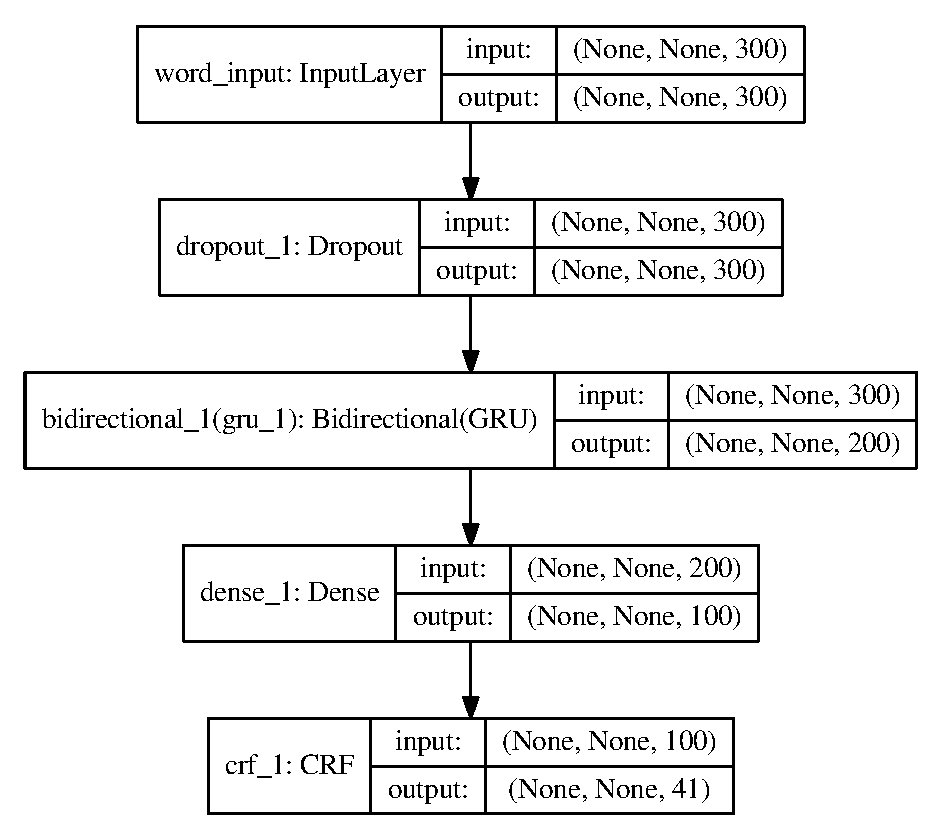
\includegraphics[width=200px]{model.eps}
\end{frame}

%----------------------------------------------------------------

\begin{frame}
    \frametitle{Word embeddings}
    \scriptsize
    \begin{tabular}{l|l|l|l|l}
        \textbf{Name} & \textbf{Corpus} & \textbf{Dim.} & \textbf{Method} & \textbf{Min count} \\
        \hline
        cc.pl.300.bin\footnote{\tiny\url{https://github.com/facebookresearch/fastText}}  & Common Crawl & 300 & CBOW     & ? \\
        kgr10-plain-sg-300-mC50.bin\footnote{\tiny\url{https://nextcloud.clarin-pl.eu/index.php/s/HIFaRv7ekgw24F1/download}} & KGR10           & 300 & skipgram & 50\\
        kgr10\_orths.vec.bin\footnote{\tiny\url{https://clarin-pl.eu/dspace/handle/11321/600}}        & KGR10           & 100 & skipgram & 5\\
    \end{tabular}
    \vspace{1em}\\
    Common features:
    \begin{itemize}
        \item fastText with character-level embeddings,
        \item simple tokenization --- not aligned with NKJP tokenization.
    \end{itemize}
    Corpora:
    \begin{itemize}
        \item Common Crawl --- Polish texts from Common Crawl\footnote{\tiny\url{http://commoncrawl.org}},
        \item KGR10 --- a corpus of Polish texts containing 4 billion words.
    \end{itemize}
\end{frame}

%----------------------------------------------------------------
    

%################################################################
\section{Evaluation}
%################################################################

\begin{frame}
    \begin{center}
        \Huge
        Evaluation
    \end{center}
\end{frame}
%----------------------------------------------------------------

\begin{frame}
    \frametitle{PolEval 2018 Task 2 official evaluation}
  \begin{table}[ht]
      \scriptsize
      \centering
      \begin{tabular}{l|c|c|c}
	  \textbf{System}	
	  & \hspace{0.2em} \textbf{Exact} \hspace{0.2em} 
	  & \hspace{0.2em} \textbf{Overlap} \hspace{0.2em} 
	  & \hspace{0.2em} \textbf{Final} \hspace{0.2em}\\
	  \hline
	  \hline
	  Per group LSTM-CRF 	& 0.826	 & 0.877 & 0.866 \\
	  \textbf{PolDeepNer}	& \textbf{0.822} & \textbf{0.859} &	\textbf{0.851} \\
	  \textbf{Liner2}	        & \textbf{0.778} & \textbf{0.818} & \textbf{0.810} \\
	  OPI\_Z3                 & 0.749 & 0.805 & 0.793 \\
	  joint	                & 0.748	& 0.789	& 0.780 \\
	  disjoint	        & 0.747	& 0.788	& 0.779 \\
	  via\_ner	        & 0.692	& 0.773	& 0.756 \\
	  kner\_sep	        & 0.700	& 0.742	& 0.733 \\
	  Poleval2k18	        & 0.623	& 0.743	& 0.719 \\
	  KNER	 	        & 0.681	& 0.719	& 0.711 \\
	  simple\_ner	        & 0.569	& 0.653	& 0.636 \\
      \end{tabular}
      \label{tab:poleval-task2-results}
  \end{table}    
\end{frame}
%----------------------------------------------------------------

%----------------------------------------------------------------


\begin{frame}
    \begin{center}
        \Huge
        Deep Learning
        
        \normalsize
        vs.
        
        \Huge
        Conditional Random Fields
        
    \end{center}
\end{frame}

%----------------------------------------------------------------

\begin{frame}
    \frametitle{Accuracy vs. Algorithmic efficiency}
    \begin{itemize}
        \item \textbf{accuracy} according to PolEval evaluation procedure, 
        \item \textbf{processing time} --- how long the evaluation dataset is being processed (in seconds), 
        \item \textbf{model size} --- total size of the model and external resources required to process the documents,
        \item \textbf{memory usage} --- total amount of memory required by the operating system (Ubuntu 16.04) to run the tool and process the documents.
    \end{itemize}
    
\begin{table}[ht]
\tiny
    \centering
    \bgroup
    \def\arraystretch{1.2}%  1 is the default, change whatever you need
    \begin{tabular}{lr|r|r|r}
                         &     &  \textbf{Liner2} & \textbf{BiLSTM-CRF} & \textbf{PolDeepNer} \\
        \hline
        \hline
        Score                  & [\%] &  81.0   &  83.9 & 85.3 \\
        \hline
        Processing speed       & [s]  &  173    &  164  & 535 \\
        \hline
        Model size             & [GB] &  0.43  & 7.20  &  16.3 \\
        \hline
        Memory usage           & [GB] & 1       & 7.3   & 17.2 \\
    \end{tabular}
    \egroup
    \label{tab:comparision}
\end{table}    
\end{frame}

\begin{frame}
    \frametitle{Accuracy vs. Algorithmic efficiency}
      \centering
      \begin{tikzpicture}
	  \tkzKiviatDiagram[scale=0.5, transform shape,label distance=.5cm,
		  radial  = 4,
		  gap     = 1,  
		  lattice = 5]{Score,Processing speed,Model size,Memory usage}
	  \tkzKiviatLine[thick,color=Plum,mark=none,fill=Plum!20,opacity=.5](4.05,1.44,0.143,0.25)
	  \tkzKiviatLine[thick,color=red,mark=none,fill=red!20,opacity=.3,dash dot](4.195,1.367,2.4,2.43)
	  \tkzKiviatLine[thick,color=blue,mark=none,fill=blue!20,opacity=.2,dash pattern={on 7pt off 2pt on 1pt off 2pt on 1pt off 3pt}](4.265,4.46,5.43,4.3)
	  \tkzKiviatGrad[prefix=,unity=20,suffix=\%](0)  
	  \tkzKiviatGrad[prefix=,unity=120,suffix=\ s](1)
	  \tkzKiviatGrad[prefix=,unity=3,suffix=\ GB](2)
	  \tkzKiviatGrad[prefix=,unity=4,suffix=\ GB](3)  
	  \node[anchor=south west,xshift=-60pt,yshift=40pt] at (current bounding box.south east) 
	  {
	  %\begin{tabular}{@{}lp{4cm}@{}}
	  \begin{tikzpicture}
	    \draw [thick,color=Plum] (0,0.2) -- (1,0.2);
	    \node[draw=none,draw=white] (A) at (1,0) {Liner2};
	    
	    \draw [thick,color=red,dash dot] (0,-0.3) -- (1,-0.3);
	    \node[draw=none,draw=white,dash dot] (B) at (1,-0.5) {BiLSTM-CRF};
	    
	    \draw [thick,color=blue,dash pattern={on 7pt off 2pt on 1pt off 2pt on 1pt off 3pt}] (0,-0.8) -- (1,-0.8);
	    \node[draw=none,draw=white] (B) at (1,-1.0) {PolDeepNer};
	    
	    \end{tikzpicture}
	  };
      \end{tikzpicture}
\end{frame}
%----------------------------------------------------------------

%################################################################
\section{The end}
%################################################################
\subsection{Summary}
\begin{frame}
  \frametitle{Summary}
  \begin{enumerate}
  	\item ...
  \end{enumerate}  
\end{frame} 

%---------------------------------------------------------------

\begin{frame}
    \centering
    \vspace{6em}
    
    Thank you for your attention.
    
    \vspace{6em}
    \pgfuseimage{pwrlogoduze}
    
    \scriptsize
    \begin{center}
    Work financed as part of the investment in the CLARIN-PL research infrastructure funded by the Polish Ministry of Science and Higher Education.
    \end{center}
\end{frame}
  
%---------------------------------------------------------------

\begin{frame}
\tiny
\bibliographystyle{plain}
\bibliography{poleval2018-poldeepner-liner2}
\end{frame}  

%---------------------------------------------------------------
  
\end{document}
